\documentclass[11pt,a4paper,dvipsnames,twosided]{article}
\usepackage[deliverable]{IOHKCoverPage}

% data for Deliverable header -- added by KH from an EU H2020 project template
%\DeliverableNumber{SL-D5}
\DeliverableTitle{A Formal Specification of the Cardano Consensus}{Formal Cardano Consensus Spec.}
\DeliverableResponsible{Formal Methods Team}
\EditorName{Javier D\'{i}az, \IOHK}
\Authors{Javier D\'{i}az \quad \texttt{<javier.diaz@iohk.io>}
%   \\[1em]
%   Polina Vinogradova \quad \texttt{<polina.vinogradova@iohk.io>}
%   \\[1em]
%   Matthias G\"udemann \quad \texttt{<matthias.gudemann@iohk.io>}
}
%\DueDate{15$^{\textrm{th}}$ October 2019}
%\SubmissionDate{8th October 2019}{2019/10/08}
\LeaderName{James Chapman, \IOHK}
\InstitutionAddress{\IOHK}
\Version{1.0}
%\Project{Shelley Ledger}
\DisseminationPU

\usepackage[margin=2.5cm]{geometry}
\usepackage{lscape}
\usepackage{iohk}
\usepackage{microtype}
\usepackage{mathpazo} % nice fonts
\usepackage{amsmath}
\usepackage{amssymb}
\usepackage{amsthm}
\usepackage{latexsym}
\usepackage{mathtools}
\usepackage{stmaryrd}
\usepackage{extarrows}
\usepackage{slashed}
\usepackage[unicode=true,pdftex,pdfa,colorlinks=true]{hyperref}
\usepackage{xcolor}
\usepackage[capitalise,noabbrev,nameinlink]{cleveref}
\usepackage{float}
\floatstyle{boxed}
\restylefloat{figure}
\usepackage{tikz}
\usepackage{booktabs}
\usepackage{enumerate}
\usepackage{listings}
%%
%% Package `semantic` can be used for writing inference rules.
%%
\usepackage{semantic}
%% Setup for the semantic package
\setpremisesspace{20pt}

\usepackage{tocloft}
\addtolength{\cftsubsecnumwidth}{5pt}

%%
%% Types
%%
\newcommand{\Nothing}{\ensuremath{\Diamond}}
\newcommand{\N}{\ensuremath{\mathbb{N}}}
\newcommand{\Bool}{\type{Bool}}
\newcommand{\Npos}{\ensuremath{\mathbb{N}^{>0}}}
\newcommand{\Z}{\ensuremath{\mathbb{Z}}}
\newcommand{\Q}{\ensuremath{\mathbb{Q}}}
\newcommand{\R}{\ensuremath{\mathbb{R}}}
\newcommand{\Rnn}{\ensuremath{\mathbb{R}^{\geq 0}}}
\newcommand{\Tx}{\type{Tx}}
\newcommand{\TxBody}{\type{TxBody}}
\newcommand{\TxWitness}{\type{TxWitness}}
\newcommand{\Ix}{\type{Ix}}
\newcommand{\TxId}{\type{TxId}}
\newcommand{\Addr}{\type{Addr}}
\newcommand{\UTxO}{\type{UTxO}}
\newcommand{\Wdrl}{\type{Wdrl}}
\newcommand{\Coin}{\type{Coin}}
\newcommand{\PParams}{\type{PParams}}
\newcommand{\PParamsUpdate}{\type{PParamsUpdate}}
\newcommand{\ProposedPPUpdates}{\type{ProposedPPUpdates}}
\newcommand{\Slot}{\type{Slot}}
\newcommand{\RandomnessStabilisationWindow}{\ensuremath{\mathsf{RandomnessStabilisationWindow}}}
\newcommand{\SlotsPerEpoch}{\mathsf{SlotsPerEpoch}}
\newcommand{\SlotsPerKESPeriod}{\mathsf{SlotsPerKESPeriod}}
\newcommand{\MaxMajorPV}{\mathsf{MaxMajorPV}}
\newcommand{\ActiveSlotCoeff}{\mathsf{ActiveSlotCoeff}}
\newcommand{\Network}{\mathsf{Network}}
\newcommand{\NetworkId}{\mathsf{NetworkId}}
\newcommand{\BlockNo}{\type{BlockNo}}
\newcommand{\MaxKESEvo}{\ensuremath{\mathsf{MaxKESEvo}}}
\newcommand{\Quorum}{\ensuremath{\mathsf{Quorum}}}
\newcommand{\MaxLovelaceSupply}{\ensuremath{\mathsf{MaxLovelaceSupply}}}
\newcommand{\Duration}{\type{Duration}}
\newcommand{\StakePools}{\type{StakePools}}
\newcommand{\Seed}{\type{Seed}}
\newcommand{\seedOp}{\star}
\newcommand{\Ppm}{\type{Ppm}}
\newcommand{\ProtVer}{\ensuremath{\type{ProtVer}}}
\newcommand{\Metadatum}{\ensuremath{\type{Metadatum}}}
\newcommand{\Metadata}{\ensuremath{\type{Metadata}}}
\newcommand{\MetadataHash}{\ensuremath{\type{MetadataHash}}}
\newcommand{\Update}{\type{Update}}
\newcommand{\GenesisDelegation}{\type{GenesisDelegation}}
\newcommand{\FutGenesisDelegation}{\type{FutGenesisDelegation}}

\newcommand{\DCert}{\type{DCert}}
\newcommand{\DCertRegKey}{\type{DCert_{regkey}}}
\newcommand{\DCertDeRegKey}{\type{DCert_{deregkey}}}
\newcommand{\DCertDeleg}{\type{DCert_{delegate}}}
\newcommand{\DCertRegPool}{\type{DCert_{regpool}}}
\newcommand{\DCertRetirePool}{\type{DCert_{retirepool}}}
\newcommand{\DCertGen}{\type{DCert_{genesis}}}
\newcommand{\DCertMir}{\type{DCert_{mir}}}
\newcommand{\PoolParam}{\type{PoolParam}}
\newcommand{\PoolMD}{\type{PoolMD}}
\newcommand{\MIRPot}{\type{MIRPot}}
\newcommand{\InstantaneousRewards}{\type{InstantaneousRewards}}
\newcommand{\ReservesMIR}{\type{ReservesMIR}}
\newcommand{\TreasuryMIR}{\type{TreasuryMIR}}
\newcommand{\URL}{\type{Url}}
\newcommand{\UTxOState}{\ensuremath{\type{UTxOState}}}
\newcommand{\ledgerState}{\ensuremath{\type{ledgerState}}}

\newcommand{\AddrRWD}{\type{Addr_{rwd}}}
\newcommand{\AddrB}{\type{Addr_{base}}}
\newcommand{\AddrP}{\type{Addr_{ptr}}}
\newcommand{\AddrE}{\type{Addr_{enterprise}}}
\newcommand{\AddrBS}{\type{Addr_{bootstrap}}}
\newcommand{\Ptr}{\type{Ptr}}
\newcommand{\DState}{\type{DState}}
\newcommand{\DWEnv}{\type{DWEnv}}
\newcommand{\DPSEnv}{\type{DPSEnv}}
\newcommand{\DPEnv}{\type{DPEnv}}
\newcommand{\DEnv}{\type{DEnv}}
\newcommand{\PEnv}{\type{PEnv}}
\newcommand{\DPState}{\type{DPState}}
\newcommand{\PState}{\type{PState}}
\newcommand{\DCertBody}{\type{DCertBody}}
\newcommand{\TData}{\type{TData}}
\newcommand{\DPoolReap}{\ensuremath{\type{poolreap}}}
\newcommand{\UPIState}{\type{UPIState}}
\newcommand{\UpdatePayload}{\type{UpdatePayload}}

% multi-signature
\newcommand{\StakeCredential}{\type{Credential}_{stake}}

\newcommand{\txwitsVKey}[1]{\fun{txwitsVKey}~\var{#1}}
\newcommand{\txwitsScript}[1]{\fun{txwitsScript}~\var{#1}}

\newcommand{\AddrVKey}{\type{Addr^{vkey}}}
\newcommand{\AddrRWDVKey}{\type{Addr_{rwd}^{vkey}}}
\newcommand{\AddrRWDScr}{\type{Addr_{rwd}^{script}}}
\newcommand{\AddrVKeyB}{\type{Addr^{vkey}_{base}}}
\newcommand{\AddrVKeyP}{\type{Addr^{vkey}_{ptr}}}
\newcommand{\AddrVKeyE}{\type{Addr^{vkey}_{enterprise}}}
\newcommand{\AddrVKeyBS}{\type{Addr^{vkey}_{bootstrap}}}
\newcommand{\AddrScr}{\type{Addr^{script}}}
\newcommand{\AddrScrBase}{\type{Addr_{base}^{script}}}
\newcommand{\AddrScrEnterprise}{\type{Addr_{enterprise}^{script}}}
\newcommand{\AddrScrPtr}{\type{Addr_{ptr}^{script}}}
\newcommand{\HashScr}{\type{ScriptHash}}
\newcommand{\Script}{\type{Script}}
\newcommand{\MSig}{\type{MSig}}
\newcommand{\Credential}{\type{Credential}}

%% Adding witnesses
\newcommand{\TxIn}{\type{TxIn}}
\newcommand{\TxOut}{\type{TxOut}}
\newcommand{\VKey}{\type{VKey}}
\newcommand{\VKeyEv}{\type{VKey_{ev}}}
\newcommand{\VKeyGen}{\type{VKey_G}}
\newcommand{\SKey}{\type{SKey}}
\newcommand{\SKeyEv}{\type{SKey_{ev}}}
\newcommand{\KeyHash}{\type{KeyHash}}
\newcommand{\KeyHashGen}{\type{KeyHash_G}}
\newcommand{\KeyPair}{\type{KeyPair}}
\newcommand{\KeyPairEv}{\type{KeyPair_{ev}}}
\newcommand{\Sig}{\type{Sig}}
\newcommand{\Data}{\type{Data}}
\newcommand{\Ser}{\type{Ser}}
%% Adding delegation
\newcommand{\Epoch}{\type{Epoch}}
\newcommand{\KESPeriod}{\type{KESPeriod}}
%% Blockchain
\newcommand{\Acnt}{\type{Acnt}}
\newcommand{\Gkeys}{\var{G_{keys}}}
\newcommand{\Block}{\type{Block}}
\newcommand{\SlotId}{\type{SlotId}}
\newcommand{\PPUpdateState}{\type{PPUpdateState}}
\newcommand{\PPUpdateEnv}{\type{PPUpdateEnv}}
\newcommand{\UTxOEnv}{\type{UTxOEnv}}
\newcommand{\CEEnv}{\type{CEEnv}}
\newcommand{\CEState}{\type{CEState}}
\newcommand{\BDEnv}{\type{BDEnv}}
\newcommand{\BDState}{\type{BDState}}
\newcommand{\LEnv}{\type{LEnv}}
\newcommand{\LState}{\type{LState}}

\newcommand{\Proof}{\type{Proof}}
\newcommand{\Seedl}{\mathsf{Seed}_\ell}
\newcommand{\Seede}{\mathsf{Seed}_\eta}
\newcommand{\slotToSeed}[1]{\fun{slotToSeed}~ \var{#1}}
\newcommand{\prevHashToNonce}[1]{\fun{prevHashToNonce}~ \var{#1}}
\newcommand{\isOverlaySlot}[3]{\fun{isOverlaySlot}~\var{#1}~\var{#2}~\var{#3}}
\newcommand{\classifyOverlaySlot}[5]{\fun{classifyOverlaySlot}~\var{#1}~\var{#2}~\var{#3}~\var{#4}~\var{#5}}

\newcommand{\T}{\type{T}}
\newcommand{\vrf}[3]{\fun{vrf}_{#1} ~ #2 ~ #3}
\newcommand{\verifyVrf}[4]{\fun{verifyVrf}_{#1} ~ #2 ~ #3 ~#4}

\newcommand{\HashHeader}{\type{HashHeader}}
\newcommand{\HashBBody}{\type{HashBBody}}
\newcommand{\bhHash}[1]{\fun{bhHash}~ \var{#1}}
\newcommand{\bHeaderSize}[1]{\fun{bHeaderSize}~ \var{#1}}
\newcommand{\bSize}[1]{\fun{bSize}~ \var{#1}}
\newcommand{\bBodySize}[1]{\fun{bBodySize}~ \var{#1}}
\newcommand{\OCert}{\type{OCert}}
\newcommand{\BHeader}{\type{BHeader}}
\newcommand{\BHBody}{\type{BHBody}}

\newcommand{\bheader}[1]{\fun{bheader}~\var{#1}}
\newcommand{\hsig}[1]{\fun{hsig}~\var{#1}}
\newcommand{\bprev}[1]{\fun{bprev}~\var{#1}}
\newcommand{\bhash}[1]{\fun{bhash}~\var{#1}}
\newcommand{\bvkcold}[1]{\fun{bvkcold}~\var{#1}}
\newcommand{\bseedl}[1]{\fun{bseed}_{\ell}~\var{#1}}
\newcommand{\bprfn}[1]{\fun{bprf}_{n}~\var{#1}}
\newcommand{\bseedn}[1]{\fun{bseed}_{n}~\var{#1}}
\newcommand{\bprfl}[1]{\fun{bprf}_{\ell}~\var{#1}}
\newcommand{\bocert}[1]{\fun{bocert}~\var{#1}}
\newcommand{\bnonce}[1]{\fun{bnonce}~\var{#1}}
\newcommand{\bleader}[1]{\fun{bleader}~\var{#1}}
\newcommand{\hBbsize}[1]{\fun{hBbsize}~\var{#1}}
\newcommand{\bbodyhash}[1]{\fun{bbodyhash}~\var{#1}}
\newcommand{\overlaySchedule}[3]{\fun{overlaySchedule}~\var{#1}~\var{#2}~\var{#3}}

\newcommand{\OCertEnv}{\type{OCertEnv}}
\newcommand{\PrtclState}{\type{PrtclState}}
\newcommand{\PrtclEnv}{\type{PrtclEnv}}
\newcommand{\OverlayEnv}{\type{OverlayEnv}}
\newcommand{\VRFState}{\type{VRFState}}
\newcommand{\TickNonceState}{\type{TickNonceState}}
\newcommand{\TickNonceEnv}{\type{TickNonceEnv}}
\newcommand{\NewEpochState}{\type{NewEpochState}}
\newcommand{\UpdateNonceState}{\type{UpdateNonceState}}
\newcommand{\UpdateNonceEnv}{\type{UpdateNonceEnv}}
\newcommand{\PoolDistr}{\type{PoolDistr}}
\newcommand{\BBodyEnv}{\type{BBodyEnv}}
\newcommand{\BBodyState}{\type{BBodyState}}
\newcommand{\RUpdEnv}{\type{RUpdEnv}}
\newcommand{\ChainEnv}{\type{ChainEnv}}
\newcommand{\ChainState}{\type{ChainState}}
\newcommand{\ChainSig}{\type{ChainSig}}
\newcommand{\LastAppliedBlock}{\type{LastAppliedBlock}}
\newcommand{\lastAppliedHash}[1]{\fun{lastAppliedHash}~\var{#1}}


%%
%% Functions
%%
\newcommand{\txins}[1]{\fun{txins}~ \var{#1}}
\newcommand{\txouts}[1]{\fun{txouts}~ \var{#1}}
\newcommand{\txcerts}[1]{\fun{txcerts}~ \var{#1}}
\newcommand{\txid}[1]{\fun{txid}~ \var{#1}}
\newcommand{\outs}[1]{\fun{outs}~ \var{#1}}
\newcommand{\values}[1]{\fun{values}~ #1}
\newcommand{\ubalance}[1]{\fun{ubalance}~ \var{#1}}
\newcommand{\txttl}[1]{\fun{txttl}~ \var{#1}}
\newcommand{\firstSlot}[1]{\fun{firstSlot}~ \var{#1}}
\newcommand{\totalDeposits}[3]{\fun{totalDeposits}~ \var{#1} ~ \var{#2} ~ \var{#3}}
\newcommand{\keyRefund}[6]{\fun{keyRefund}~ {#1}~{#2}~{#3}~\var{#4}~\var{#5}~\var{#6}}
\newcommand{\refund}[4]{\fun{refund}~ \var{#1}~ \var{#2}~ {#3}~ {#4}}
\newcommand{\keyRefunds}[2]{\fun{keyRefunds}~ \var{#1}~ \var{#2}}
\newcommand{\consumed}[2]{\fun{consumed}~ \var{#1}~ \var{#2}}
\newcommand{\produced}[2]{\fun{produced}~ \var{#1}~ \var{#2}}
\newcommand{\applyFun}[2]{\fun{#1}~\var{#2}}

\newcommand{\RegKey}[1]{\textsc{RegKey}(#1)}
\newcommand{\DeregKey}[1]{\textsc{DeregKey}(#1)}
\newcommand{\Delegate}[1]{\textsc{Delegate}(#1)}
\newcommand{\RegPool}[1]{\textsc{RegPool}(#1)}
\newcommand{\RetirePool}[1]{\textsc{RetirePool}(#1)}
\newcommand{\cwitness}[1]{\fun{cwitness}~ \var{#1}}
\newcommand{\dpool}[1]{\fun{dpool}~ \var{#1}}
\newcommand{\poolParam}[1]{\fun{poolParam}~ \var{#1}}
\newcommand{\retire}[1]{\fun{retire}~ \var{#1}}
\newcommand{\addrRw}[1]{\fun{addr_{rwd}}~ \var{#1}}
\newcommand{\epoch}[1]{\fun{epoch}~\var{#1}}
\newcommand{\kesPeriod}[1]{\fun{kesPeriod}~\var{#1}}

%% UTxO witnesses
\newcommand{\inputs}[1]{\fun{inputs}~ \var{#1}}
\newcommand{\txwits}[1]{\fun{txwits}~ \var{#1}}
\newcommand{\verify}[3]{\fun{verify} ~ #1 ~ #2 ~ #3}
\newcommand{\sign}[2]{\fun{sign} ~ #1 ~ #2}
\newcommand{\verifyEv}[4]{\fun{verify_{ev}} ~ #1 ~ #2 ~ #3 ~ #4}
\newcommand{\signEv}[3]{\fun{sign_{ev}} ~ #1 ~ #2 ~ #3}
\newcommand{\serialised}[1]{\llbracket \var{#1} \rrbracket}
\newcommand{\hashKey}[1]{\fun{hashKey}~ \var{#1}}
\newcommand{\txbody}[1]{\fun{txbody}~ \var{#1}}
\newcommand{\txfee}[1]{\fun{txfee}~ \var{#1}}
\newcommand{\txwdrls}[1]{\fun{txwdrls}~ \var{#1}}
\newcommand{\minfee}[2]{\fun{minfee}~ \var{#1}~ \var{#2}}
\newcommand{\slotminus}[2]{\var{#1}~-_{s}~\var{#2}}
\DeclarePairedDelimiter\floor{\lfloor}{\rfloor}
% wildcard parameter
\newcommand{\wcard}[0]{\rule[-.5mm]{2mm}{.2mm}}
%% Adding ledgers...
\newcommand{\utxo}[1]{\fun{utxo}~ #1}
%% Delegation
\newcommand{\delegatesName}{\fun{delegates}}
\newcommand{\delegates}[3]{\delegatesName~#1~#2~#3}
\newcommand{\dwho}[1]{\fun{dwho}~\var{#1}}
\newcommand{\depoch}[1]{\fun{depoch}~\var{#1}}
\newcommand{\dval}{\ensuremath{d_{\mathsf{val}}}}
%% Delegation witnesses
\newcommand{\dbody}[1]{\fun{dbody}~\var{#1}}
\newcommand{\dwit}[1]{\fun{dwit}~\var{#1}}
%% Blockchain
\newcommand{\bwit}[1]{\fun{bwit}~\var{#1}}
\newcommand{\bslot}[1]{\fun{bslot}~\var{#1}}
\newcommand{\bblockno}[1]{\fun{bblockno}~\var{#1}}
\newcommand{\bbody}[1]{\fun{bbody}~\var{#1}}
\newcommand{\bhbody}[1]{\fun{bhbody}~\var{#1}}
\newcommand{\bdlgs}[1]{\fun{bdlgs}~\var{#1}}
%% ledgerstate constants
\newcommand{\genesisId}{\ensuremath{Genesis_{Id}}}
\newcommand{\genesisTxOut}{\ensuremath{Genesis_{Out}}}
\newcommand{\genesisUTxO}{\ensuremath{Genesis_{UTxO}}}
\newcommand{\genesisUTxOState}{(\genesisUTxO,\wcard,\wcard,\wcard)}
\newcommand{\emax}{\ensuremath{\mathsf{E_{max}}}}

\newcommand{\unitInterval}{\ensuremath{[0,~1]}}
\newcommand{\unitIntervalNonNull}{\ensuremath{(0,~1]}}
\newcommand{\nonnegReals}{\ensuremath{[0,~\infty)}}
\newcommand{\posReals}{\ensuremath{(0,~\infty)}}

\theoremstyle{definition}
\newtheorem{definition}{Definition}[section]
\newtheorem{lemma}[definition]{Lemma}
\newtheorem{theorem}[definition]{Theorem}
\newtheorem{property}{Property}[section]

\newcommand{\leteq}{\ensuremath{\mathrel{\mathop:}=}}

\begin{document}

\hypersetup{
  pdftitle={A Formal Specification of the Cardano Consensus},
  breaklinks=true,
  bookmarks=true,
  colorlinks=false,
  linkcolor={blue},
  citecolor={blue},
  urlcolor={blue},
  linkbordercolor={white},
  citebordercolor={white},
  urlbordercolor={white}
}

  \cleardoublepage%
  \tableofcontents%

  \listoffigures%
  \clearpage%

  \begin{changelog}
        \change{2024/03/01}{Javier D\'{i}az}{FM (IOHK)}{Initial version (0.1).}
  \end{changelog}
      \clearpage%
\renewcommand{\thepage}{\arabic{page}}
\setcounter{page}{1}

\title{A Formal Specification of the Cardano Consensus}

\author{Javier D\'{i}az  \\ {\small \texttt{javier.diaz@iohk.io}}}

%\date{}

\maketitle

\begin{abstract}
This document provides a formal specification of the Cardano consensus layer.
\end{abstract}

\section*{List of Contributors}
\label{acknowledgements}

...

\cleardoublepage%
%\tableofcontents%

%\chapter{Introduction}

The Cardano Consensus and Storage layer, or \emph{the consensus layer} for
short, is a critical piece of infrastructure in the Cardano Node. It
orchestrates between the \emph{network layer} below it and the
\emph{ledger layer} above it.

The network layer is a highly concurrent piece of software that deals with
low-level concerns; its main responsibility is to transmit data efficiently
across the network. Although it primarily transmits blocks and block headers, it
does not interpret them and does not need to know much about them. In the few
cases where it \emph{does} need to make some block-specific decisions, it
calls back into the consensus layer to do so.

The ledger layer by contrast exclusively deals with high-level concerns. It is
entirely stateless: its main responsibility is to define a single pure
function describing how the ledger state is transformed by blocks (verifying
that blocks are valid in the process). It is only concerned with linear history;
it is not aware of the presence of multiple competing chains or the roll backs
required when switching from one chain to another. We do require that the ledger
layer provides limited \emph{lookahead}, computing (views on near)
\emph{future} ledger states (required to be able to validate block headers
without access to the corresponding block bodies)

The consensus layer mediates between these two layers. It includes a
bespoke storage layer that provides efficient access to the current ledger state
as well as recent \emph{past} ledger states (required in order to be able
to validate and switch to competing chains). The storage layer also
provides direct access to the blocks on the blockchain itself, so that they can
be efficiently streamed to clients (via the network layer). When there are
competing chains, the consensus layer decides which chain is preferable and
should be adopted, and it decides when to \emph{contribute} to the chain
(produce new blocks). All ``executive decisions'' about the chain are made in
and by the consensus layer.

Lastly, as well we see, the consensus layer is highly abstract and places a
strong emphasis on compositionality, making it usable with many different
consensus algorithms and ledgers. Importantly, compositionality enables the
\emph{hard fork combinator} to combine multiple ledgers and regard them as a
single blockchain.

The goal of this document is to outline the design goals for the consensus
layer, how we achieved them, and where there is still scope for improvement. We
will both describe \emph{what} the consensus layer is, and \emph{why} it is the
way it is. Throughout we will also discuss what \emph{didn't} work, approaches
we considered but rejected, or indeed adopted but later abandoned; discussing
these dead ends is sometimes at least as informative as discussing the solution
that did work.

We will consider some of the trade-offs we have had to make, how they
affected the development, and discuss which of these trade-offs should perhaps
be reconsidered. We will also take a look at how the design can scale to
facilitate future requirements, and which requirements will be more problematic
and require more large-scale refactoring.

The target audience for this document is primarily developers working on the
consensus layer. It may also be of more broader interest to people generally
interested in the Cardano blockchain, although we will assume that the
reader has a technical background.

%\include{notation}
%\include{crypto-primitives}
%\include{address}
%\include{protocol-parameters}
%\include{transactions}
%\include{update}
%\include{utxo}
%\include{delegation}
%\chapter{Interface to the ledger}
\label{ledger}

\section{Abstract interface}
\label{ledger:api}

In \cref{overview:ledger} we identified three responsibilities for the ledger
layer:
%
\begin{itemize}
\item ``Ticking'' the ledger state, applying any time related changes
(\cref{ledger:api:IsLedger}). This is independent from blocks, both at the value
level (we don't need a block in order to tick) and at the type level.
\item Applying and verifying blocks (\cref{ledger:api:ApplyBlock}). This
obviously connects a ledger and a block type, but we try to avoid to talk about
\emph{the} ledger corresponding to a block, in order to improve
compositionality; we will see examples of where this comes in useful in the
definition of the extended ledger state (\cref{storage:extledgerstate}) and the
ledger database (\cref{ledgerdb}).
\item Projecting out the ledger view (\cref{ledger:api:LedgerSupportsProtocol}),
connecting a ledger to a consensus protocol.
\end{itemize}
%
We will discuss these responsibilities one by one.

\subsection{Independent definitions}
\label{ledger:api:IsLedger}

We will start with ledger API that can be defined independent of a choice of
block or a choice of consensus protocol.

\subsubsection{Configuration}

Like the other abstractions in the consensus layer, the ledger defines its own
type of required static configuration
%
\begin{lstlisting}
type family LedgerCfg l :: Type
\end{lstlisting}

\subsubsection{Tip}

We require that any ledger can report its tip as a \lstinline!Point!. A
\lstinline!Point! is either genesis (no blocks have been applied yet) or a pair
of a hash and slot number; it is parametric over $l$ in order to allow
different ledgers to use different hash types.
%
\begin{lstlisting}
class GetTip l where
  getTip :: l -> Point l
\end{lstlisting}

\subsubsection{Ticking}

We can now define the \lstinline!IsLedger! class as
%
\begin{lstlisting}
class (GetTip l, GetTip (Ticked l), ..) => IsLedger l where
  type family LedgerErr l :: Type
  applyChainTick :: LedgerCfg l -> SlotNo -> l -> Ticked l
\end{lstlisting}

The type of \lstinline!applyChainTick! is similar to the type of
\lstinline!tickChainDepState! we saw in \cref{consensus:class:state}.
Examples of the time-based changes in the ledger state include activating
delegation certificates in the Byron ledger, or paying out staking rewards
in the Shelley ledger.

Ticking is not allowed to fail (it cannot return an error). Consider what it
would mean if it \emph{could} fail: it would mean that a previous block was
accepted as valid, but set up the ledger state so that no matter what would
happen next, as soon as a particular moment in time is reached, the ledger would
fail to advance any further. Obviously, such a situation cannot be permitted to
arise (the block should have been rejected as invalid).

Note that ticking does not change the tip of the ledger: no blocks have been
applied (yet). This means that we should have

\begin{equation}
  \mathtt{getTip} \; l
= \mathtt{getTip} \; (\mathtt{applyChainTick}_\mathit{cfg} \; s \; l)
\end{equation}

\subsubsection{Ledger errors}

The inclusion of \lstinline!LedgerErr! in \lstinline!IsLedger! is perhaps
somewhat surprising. \lstinline!LedgerErr! is the type of errors that can arise
when applying blocks to the ledger, but block application is not yet defined
here. Nonetheless, a ledger can only be used with a \emph{single} type of
block\footnote{While it is true that the Cardano ledger can be used with Byron
blocks, Shelley blocks, Goguen blocks, etc., this distinction between the
different blocks is invisible to most of the consensus layer. The whole raison
d'\^{e}tre of the hard fork combinator (\cref{hfc}) is to present a composite
ledger (say, the one consisting of the Byron, Shelley and Goguen eras) as a
single type of ledger with a single type of block. The rest of the consensus
layer is not aware that this composition has happened; from its point
perspective it's just another ledger with an associated block type.}, and
consequently can only have a \emph{single} type of error; the only reason block
application is defined separately is that a single type of \emph{block} can be
used with multiple ledgers (in other words, this is a 1-to-many
relationship).\footnote{Defining \lstinline!LedgerErr! in \lstinline!ApplyBlock!
(\cref{ledger:api:ApplyBlock}) would result in ambiguous types, since it would
not refer to the \lstinline!blk! type variable of that class.}

\subsection{Applying blocks}
\label{ledger:api:ApplyBlock}

If \lstinline!applyChainTick! was analogous to \lstinline!tickChainDepState!,
then \lstinline!applyLedgerBlock! and \lstinline!reapplyLedgerBlock! are
analogous to \lstinline!updateChainDepState! and
\lstinline!reupdateChainDepState!, respectively
(\cref{consensus:class:state}): apply a block to an already ticked
ledger state:
%
\begin{lstlisting}
class (IsLedger l, ..) => ApplyBlock l blk where
  applyLedgerBlock ::
    LedgerCfg l -> blk -> Ticked l -> Except (LedgerErr l) l
  reapplyLedgerBlock ::
    LedgerCfg l -> blk -> Ticked l -> l
\end{lstlisting}
%
The discussion of the difference between, and motivation for, the distinction
between application and reapplication in \cref{consensus:class:state}
about the consensus protocol state applies here equally.

\subsection{Linking a block to its ledger}

We mentioned at the start of \cref{ledger:api} that a single block can be used
with multiple ledgers. Nonetheless, there is one ``canonical'' ledger for each
block; for example, the Shelley block is associated with the Shelley ledger,
even if it can also be applied to the extended ledger state or the ledger
DB. We express this through a data family linking a block to its ``canonical
ledger state'':
%
\begin{lstlisting}
data family LedgerState blk :: Type
\end{lstlisting}
%
and then require that it must be possible to apply a block to its associated
ledger state
%
\begin{lstlisting}
class ApplyBlock (LedgerState blk) blk => UpdateLedger blk
\end{lstlisting}
%
(this is an otherwise empty class). For convenience, we then also introduce
some shorthand:
%
\begin{lstlisting}
type LedgerConfig      blk = LedgerCfg (LedgerState blk)
type LedgerError       blk = LedgerErr (LedgerState blk)
type TickedLedgerState blk = Ticked    (LedgerState blk)
\end{lstlisting}

\subsection{Projecting out the ledger view}
\label{ledger:api:LedgerSupportsProtocol}

In \cref{overview:ledger} we mentioned that a consensus protocol may require
some information from the ledger, and in \cref{consensus:class:ledgerview} we
saw that this is modelled as the \lstinline!LedgerView! type family in the
\lstinline!ConsensusProtocol! class. A ledger and a consensus protocol are
linked through the block type (indeed, apart from the fundamental concepts we
have discussed so far, most of consensus is parameterised over blocks, not
ledgers or consensus protocols). Recall from \cref{BlockSupportsProtocol} that
the \lstinline!BlockProtocol! type family defines for each block what the
corresponding consensus protocol is; we can use this to define the projection of
the ledger view (defined by the consensus protocol) from the ledger state as
follows:
%
\begin{lstlisting}
class (..) => LedgerSupportsProtocol blk where
  protocolLedgerView ::
       LedgerConfig blk
    -> Ticked (LedgerState blk)
    -> Ticked (LedgerView (BlockProtocol blk))

  ledgerViewForecastAt ::
       LedgerConfig blk
    -> LedgerState blk
    -> Forecast (LedgerView (BlockProtocol blk))
\end{lstlisting}
%
The first method extracts the ledger view out of an already ticked ledger state;
think of it as the ``current'' ledger view. Forecasting deserves a more detailed
discussion and will be the topic of the next section.

\section{Forecasting}
\label{ledger:forecasting}

\subsection{Introduction}

In \cref{nonfunctional:network:headerbody} we discussed the need to validate
headers from upstream peers. In general, header validation requires information
from the ledger state. For example, in order to verify whether a Shelley header
was produced by the right node, we need to know the stake distribution (recall
that in Shelley the probability of being elected a leader is proportional to the
stake); this information is precisely what is captured by the
\lstinline!LedgerView! (\cref{consensus:class:ledgerview}). However, we cannot
update the ledger state with block headers only, we need the block bodies: after
all, to stay with the Shelley example, the stake evolves based on the
transactions that are made, which appear only in the block bodies.

Not all is lost, however. The stake distribution used by the Shelley ledger for
the sake of the leadership check \emph{is not the \emph{current} stake
distribution}, but the stake distribution as it was at a specific point in the
past. Moreover, that same stake distribution is then used for all leadership
checks in a given period of time.\footnote{The exact details of precisely
\emph{how} the chain is split is not relevant to the consensus layer, and is
determined by the ledger layer.} In the depiction below, the stake distribution
as it was at point $b$ is used for the leadership checks near the current tip,
the stake distribution at point $a$ was used before that, and so forth:
%
\begin{center}
\begin{tikzpicture}
%                             /--------\
%                             |        |
%                             *        v  tip
% 1 -----+------------+------------+-----+
%        |       *    |            |     * current stake
% 0 -----+------------+------------+-----|
%   -10  -8           -4           0     2
%                |          ^
%                \----------/
\draw (-10, 0.5) node{\ldots};
\draw (-10,  0) --  (2, 0);
\draw (-10,  1) --  (2, 1);
\draw  (-8,  0) -- (-8, 1);
\draw  (-4,  0) -- (-4, 1);
\draw   (0,  0) --  (0, 1);
\draw   (2,  0) --  (2, 1) node[above]{tip};
\draw  (-6, -0.2) node {$\underbrace{\hspace{3.8cm}}$};
\draw  (-2, -0.2) node {$\underbrace{\hspace{3.8cm}}$};
\draw  ( 2, -0.2) node {$\underbrace{\hspace{3.8cm}}$};
\draw [thick, arrows={-Triangle}] (-9, -1) node[fill=white] {$\ldots$}-- (-6, -1) -- (-6, -0.3);
\draw [thick, arrows={-Triangle}] (-5, 0.5) node[fill=white] {$\mathstrut a$} -- (-5, -1) -- (-2, -1) -- (-2, -0.3);
\draw [thick, arrows={-Triangle}] (-1, 0.5) node[fill=white] {$\mathstrut b$} -- (-1, -1) -- (2, -1) -- (2, -0.3);
\end{tikzpicture}
\end{center}
%
This makes it possible to \emph{forecast} what the stake distribution (i.e.,
the ledger view) will be at various points. For example, if the chain looks like
%
\begin{center}
\begin{tikzpicture}
\draw (-10,    0.5) node{\ldots};
\draw (-10,    0) -- (-0.5, 0);
\draw (-10,    1) -- (-0.5, 1);
\draw  (-8,    0) -- (-8,   1);
\draw  (-4,    0) -- (-4,   1);
\draw  (-0.5,  0) -- (-0.5, 1) node[above]{tip};
\draw  (-6,   -0.2) node {$\underbrace{\hspace{3.8cm}}$};
\draw  (-2,   -0.2) node {$\underbrace{\hspace{3.8cm}}$};
\draw  ( 2,   -0.2) node {$\underbrace{\hspace{3.8cm}}$};
\draw [thick, arrows={-Triangle}] (-9, -1) node[fill=white] {$\ldots$}-- (-6, -1) -- (-6, -0.3);
\draw [thick, arrows={-Triangle}] (-5, 0.5) node[fill=white] {$\mathstrut a$} -- (-5, -1) -- (-2, -1) -- (-2, -0.3);
\draw [thick, arrows={-Triangle}] (-1, 0.5) node[fill=white] {$\mathstrut b$} -- (-1, -1) -- (2, -1) -- (2, -0.3);
\draw (0, 0.5) node[left] {$\mathstrut c$};
\draw (0, 0.5) node[right] {$\mathstrut d$};
\draw (4, 0.5) node[right] {$\mathstrut e$};
\end{tikzpicture}
\end{center}
%
then we can ``forecast'' that the stake distribution at point $c$ will be the one
established at point $a$, whereas the stake distribution at point $d$ will be the
one established at point $b$. The stake distribution at point $e$ is however not
yet known; we say that $e$ is ``out of the forecast range''.

\subsection{Code}

Since we're always forecasting what the ledger would look like \emph{if it would
be advanced to a particular slot}, the result of forecasting is always something
ticked:\footnote{An \emph{unticked} ledger view would arise from deriving the
ledger view from the \emph{current} ledger state, not taking (nor needing to
take) into account any changes that have been scheduled for later slots. The
unticked ledger view is however rarely useful; when we validate a header, any
changes that have been scheduled in the most recent ledger state for slots
before or at the slot number of the header must be applied before we validate
the header; we therefore almost exclusively work with ticked ledger views.}
%
\begin{lstlisting}
data Forecast a = Forecast {
      forecastAt  :: WithOrigin SlotNo
    , forecastFor :: SlotNo -> Except OutsideForecastRange (Ticked a)
    }
\end{lstlisting}
%
Here \lstinline!forecastAt! is the tip of the ledger in which the forecast was
constructed and \lstinline!forecastFor! is constructing the forecast for a
particular slot, possibly returning an error message of that slot is out of
range. This terminology---a forecast constructed \emph{at} a slot
and computed \emph{for} a slot---is used throughout both this technical report
as well as the consensus layer code base.

\subsection{Ledger view}
\label{forecast:ledgerview}

For the ledger view specifically, the \lstinline!LedgerSupportsProtocol!
class (\cref{ledger:api:LedgerSupportsProtocol}) requires a function
%
\begin{lstlisting}
ledgerViewForecastAt ::
     LedgerConfig blk
  -> LedgerState blk
  -> Forecast (LedgerView (BlockProtocol blk))
\end{lstlisting}
%
This function must satisfy two important properties:
%
\begin{description}
\item[Sufficient range]

When we validate headers from an upstream node, the most recent usable ledger
state we have is the ledger state at the intersection of our chain and the chain
of the upstream node. That intersection will be at most $k$ blocks back, because
that is our maximum rollback and we disconnect from nodes that fork from our
chain more than $k$ blocks ago (\cref{consensus:overview:k}). Furthermore, it is
only useful to track an upstream peer if we might want to adopt their blocks,
and we only switch to their chain if it is longer than ours
(\cref{consensus:overview:chainsel}). This means that in the worst case
scenario, with the intersection $k$ blocks back, we need to be able to evaluate
$k + 1$ headers in order to adopt the alternative chain. However, the range of a
forecast is based on \emph{slots}, not blocks; since not every slot may contain
a block (\cref{time:slots-vs-blocks}), the range needs to be sufficient to
\emph{guarantee} to contain at least $k + 1$ blocks\footnote{Due to a
misalignment between the consensus requirements and the Shelley specification,
this is not the case for Shelley, where the effective maximum rollback is in
fact $k - 1$; see \cref{shelley:forecasting}).}; we will come back to this in
\cref{future:block-vs-slot}.

The network layer may have additional reasons for wanting a long forecast
range; see \cref{nonfunctional:network:headerbody}.

\item[Relation to ticking]
Forecasting is not the only way that we can get a ledger view for a particular
slot; alternatively, we can also \emph{tick} the ledger state, and then ask
for the ledger view at that ticked ledger state. These two ways should give us
the same answer:
%
\begin{equation}
\begin{array}{lllll}
\mathrm{whenever} &
\mathtt{forecastFor} \; (\mathtt{ledgerViewForecastAt}_\mathit{cfg} \; l) \; s & = & \mathtt{Right} & l' \\
\mathrm{then} & \mathtt{protocolLedgerView}_\mathit{cfg} \; (\mathtt{applyChainTick}_\mathit{cfg} \; s \; l) & = && l'
\end{array}
\end{equation}
%
In other words, whenever the ledger view for a particular slot is within the
forecast range, then ticking the ledger state to that slot and asking for the
ledger view at the tip should give the same answer. Unlike forecasting, however,
ticking has no maximum range. The reason is the following fundamental difference between these two concepts:
%
\begin{quote}
\textbf{(Forecast vs. ticking)} When we \emph{forecast} a ledger view, we are
predicting what that ledger view will be, \emph{no matter which blocks will  be
applied to the chain} between the current tip and the slot of the forecast. By
contrast, when we \emph{tick} a ledger, we are applying any time-related
changes to the ledger state in order to apply the \emph{next} block; in other
words, when we tick to a particular slot, \emph{there \emph{are} no blocks in
between the current tip and the slot we're ticking to}. Since there are no
intervening blocks, there is no uncertainty, and hence no limited range.
\end{quote}
\end{description}

\section{Queries}
\label{ledger:queries}

\section{Abandoned approach: historical states}

%\include{epoch}
\section{Common Interface}
\label{sec:common-interface}

This section defines the interface used by this specification, i.e.
the transition systems that are assumed to exist.

\subsection{Chain Tick Transition}
\label{sec:tick-trans}

The Chain Tick Transition performs some chain level upkeep.
\begin{figure}[htb]
  \emph{Chain Tick Transitions}
  \begin{equation*}
    \vdash \var{\_} \trans{tick}{\_} \var{\_} \subseteq
    \powerset (\NewEpochState \times \Slot \times \NewEpochState)
  \end{equation*}
  \caption{Tick transition-system types}
  \label{fig:ts-types:tick}
  %
\end{figure}

The type of the $\mathsf{TICK}$ transition is shown in Figure~\ref{fig:ts-types:tick}.

\subsection{Ledger Sequence Transition}
\label{sec:ledgers-trans}

The Ledger Sequence Transition processes a list of transactions.
\begin{figure}[htb]
  \emph{Ledger Sequence transitions}
  \begin{equation*}
    \_ \vdash
    \var{\_} \trans{ledgers}{\_} \var{\_}
    \subseteq \powerset ((\Slot\times\PParams\times\Coin) \times \LState \times \seqof{\Tx} \times \LState)
  \end{equation*}
  \caption{Ledger Sequence transition-system types}
  \label{fig:ts-types:ledgers}
\end{figure}

The type of the $\mathsf{LEDGERS}$ transition system is shown in Figure~\ref{fig:ts-types:ledgers}.

%%% Local Variables:
%%% mode: latex
%%% TeX-master: "ledger-spec"
%%% End:

\section{Transition Rule Dependencies}
\label{sec:sts-rules-overview}

Figure~\ref{fig:sts-rules-dependencies} shows all STS rules, the sub-rules they
use and possible dependencies. Each node in the graph represents one rule, the
top rule being $\mathsf{CHAINHEAD}$.\@ A straight arrow from one node to another
one represents a sub-rule relationship.

An arrow with a dotted line from one node to another represents a dependency in
the sense that the output of the target rule is an input to the source one,
either as part of the source state, the environment or the signal. In most cases
these dependencies are between sub-rules of a rule. In the case of recursive
rules, the sub-rule can also have a dependency on the super-rule. Those
recursively call themselves while traversing the input signal sequence until
reaching the base case with an empty input sequence.

\begin{figure}[htp]
  \centering
  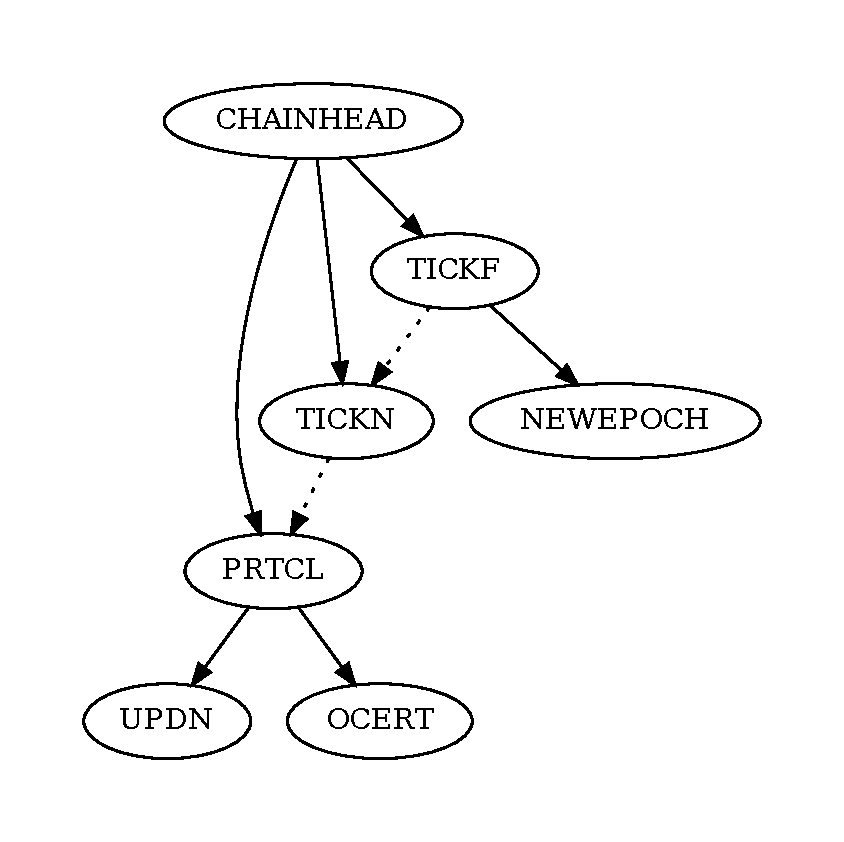
\includegraphics[width=\textwidth]{rules}
  \caption{STS Rules, Sub-Rules and Dependencies}
  \label{fig:sts-rules-dependencies}
\end{figure}


\section{Blockchain layer}
\label{sec:chain}

\newcommand{\BlocksMade}{\type{BlocksMade}}
\newcommand{\XOR}{\mathsf{XOR}}

This chapter introduces the view of the blockchain layer as required for the
consensus. The main transition rule is $\mathsf{CHAINHEAD}$ which calls the subrules
$\mathsf{TICKF}$, $\mathsf{TICKN}$ and $\mathsf{PRTCL}$.

\subsection{Block Definitions}
\label{sec:defs-blocks}

\begin{figure*}[htb]
  \emph{Abstract types}
  %
  \begin{equation*}
    \begin{array}{r@{~\in~}lr}
      \var{h} & \HashHeader & \text{hash of a block header}\\
      \var{hb} & \HashBBody & \text{hash of a block body}\\
      \var{bn} & \BlockNo & \text{block number}\\
    \end{array}
  \end{equation*}
  %
  \emph{Operational Certificate}
  %
  \begin{equation*}
    \OCert =
    \left(
      \begin{array}{r@{~\in~}lr}
        \var{vk_{hot}} & \VKeyEv & \text{operational (hot) key}\\
        \var{n} & \N & \text{certificate issue number}\\
        c_0 & \KESPeriod & \text{start KES period}\\
        \sigma & \Sig & \text{cold key signature}\\
      \end{array}
    \right)
  \end{equation*}
  %
  \emph{Block Header Body}
  %
  \begin{equation*}
    \BHBody =
    \left(
      \begin{array}{r@{~\in~}lr}
        \var{prev} & \HashHeader^? & \text{hash of previous block header}\\
        \var{vk} & \VKey & \text{block issuer}\\
        \var{vrfVk} & \VKey & \text{VRF verification key}\\
        \var{blockno} & \BlockNo & \text{block number}\\
        \var{slot} & \Slot & \text{block slot}\\
        \var{vrfRes} & \Seed & \text{VRF result value}\\
        \var{prf} & \Proof & \text{VRF proof}\\
        \var{bsize} & \N & \text{size of the block body}\\
        \var{bhash} & \HashBBody & \text{block body hash}\\
        \var{oc} & \OCert & \text{operational certificate}\\
        \var{pv} & \ProtVer & \text{protocol version}\\
      \end{array}
    \right)
  \end{equation*}
  %
  \emph{Block Types}
  %
  \begin{equation*}
    \begin{array}{r@{~\in~}l@{\qquad=\qquad}l}
      \var{bh}
      & \BHeader
      & \BHBody \times \Sig
    \end{array}
  \end{equation*}
  \emph{Abstract functions}
  %
  \begin{equation*}
    \begin{array}{r@{~\in~}lr}
      \bhHash{} & \BHeader \to \HashHeader
                   & \text{hash of a block header} \\
      \bHeaderSize{} & \BHeader \to \N
                   & \text{size of a block header} \\
      \slotToSeed{} & \Slot \to \Seed
                    & \text{convert a slot to a seed} \\
      \prevHashToNonce{} & \HashHeader^? \to \Seed
                    & \text{convert an optional header hash to a seed} \\
    \end{array}
  \end{equation*}
  %
  \emph{Accessor Functions}
  \begin{equation*}
    \begin{array}{r@{~\in~}l@{~~~~~~~~~~}r@{~\in~}lr}
      \fun{bheader} & \Block \to \BHeader &
      \fun{bhbody} & \BHeader \to \BHBody \\
      \fun{hsig} & \BHeader \to \Sig &
      \fun{bvkcold} & \BHBody \to \VKey \\
      \fun{bvkvrf} & \BHBody \to \VKey &
      \fun{bprev} & \BHBody \to \HashHeader^? \\
      \fun{bslot} & \BHBody \to \Slot &
      \fun{bblockno} & \BHBody \to \BlockNo \\
      \fun{bVrfRes} & \BHBody \to \Seed &
      \fun{bVrfProof} & \BHBody \to \Proof \\
      \fun{hBbsize} & \BHBody \to \N &
      \fun{bhash} & \BHBody \to \HashBBody \\
      \fun{bocert} & \BHBody \to \OCert \\
    \end{array}
  \end{equation*}
  %
  \caption{Block Definitions}
  \label{fig:defs:blocks}
\end{figure*}

%%
%% Figure - Helper Functions for Blocks
%%
\begin{figure}[htb]
  \emph{Block Helper Functions}
  \begin{align*}
      & \fun{bleader} \in \BHBody \to \Seed \\
      & \fun{bleader}~\var{bhb} = \fun{hash}~(``L"~|~(\fun{bVrfRes}~\var{bhb}))\\
      \\
      & \fun{bnonce} \in \BHBody \to \Seed \\
      & \fun{bnonce}~\var{bhb} = \fun{hash}~(``N"~|~(\fun{bVrfRes}~\var{bhb}))\\
  \end{align*}
  %
  \caption{Helper Functions used for Blocks}
  \label{fig:funcs:blocks-helper}
\end{figure}

\clearpage

\subsection{Tick Nonce Transition}
\label{sec:tick-nonce-trans}

The Tick Nonce Transition is responsible for updating the epoch nonce and the
previous epoch's hash nonce at the start of an epoch. Its environment is shown in
Figure~\ref{fig:ts-types:ticknonce} and consists of the protocol parameters
$\var{pp}$, the candidate nonce $\eta_c$ and the previous epoch's last block
header hash as a nonce. Its state consists of the epoch nonce $\eta_0$ and
the previous epoch's last block header hash nonce $\eta_h$.

\begin{figure}
  \emph{Tick Nonce environments}
  \begin{equation*}
    \TickNonceEnv =
    \left(
      \begin{array}{r@{~\in~}lr}
        \var{pp} & \PParams & \text{protocol parameters} \\
        \eta_c & \Seed & \text{candidate nonce} \\
        \eta_\var{ph} & \Seed & \text{previous header hash as nonce} \\
      \end{array}
    \right)
  \end{equation*}
  %
  \emph{Tick Nonce states}
  \begin{equation*}
    \TickNonceState =
    \left(
      \begin{array}{r@{~\in~}lr}
        \eta_0 & \Seed & \text{epoch nonce} \\
        \eta_h & \Seed & \text{seed from hash of previous epoch's last block header} \\
      \end{array}
    \right)
  \end{equation*}
  \label{fig:ts-types:ticknonce}
\end{figure}

The signal to the transition rule $\mathsf{TICKN}$ is a marker indicating
whether we are in a new epoch. If we are in a new epoch, we update the epoch
nonce and the previous hash. Otherwise, we do nothing.

\begin{figure}[ht]
  \begin{equation}\label{eq:tick-nonce-notnewepoch}
   \inference[Not-New-Epoch]
   { }
   {
     {\begin{array}{c}
        \var{pp} \\
        \eta_c \\
        \eta_\var{ph} \\
      \end{array}}
     \vdash
     {\left(\begin{array}{c}
           \eta_0 \\
           \eta_h \\
     \end{array}\right)}
     \trans{tickn}{\mathsf{False}}
     {\left(\begin{array}{c}
           \eta_0 \\
           \eta_h \\
     \end{array}\right)}
   }
 \end{equation}

 \nextdef

 \begin{equation}\label{eq:tick-nonce-newepoch}
   \inference[New-Epoch]
   {}
   {
     {\begin{array}{c}
        \var{pp} \\
        \eta_c \\
        \eta_\var{ph} \\
      \end{array}}
     \vdash
     {\left(\begin{array}{c}
           \eta_0 \\
           \eta_h \\
     \end{array}\right)}
     \trans{tickn}{\mathsf{True}}
     {\left(\begin{array}{c}
           \varUpdate{\eta_c \seedOp \eta_h} \\
           \varUpdate{\eta_\var{ph}} \\
     \end{array}\right)}
   }
 \end{equation}

 \caption{Tick Nonce rules}
 \label{fig:rules:tick-nonce}
\end{figure}

\subsection{Update Nonce Transition}
\label{sec:update-nonces-trans}

The Update Nonce Transition updates the nonces until the randomness gets fixed.
The environment is shown in Figure~\ref{fig:ts-types:updnonce} and consists of
the block nonce $\eta$.
The state is shown in Figure~\ref{fig:ts-types:updnonce} and consists of
the candidate nonce $\eta_c$ and the evolving nonce $\eta_v$.

\begin{figure}
  \emph{Update Nonce environments}
  \begin{equation*}
    \UpdateNonceEnv =
    \left(
      \begin{array}{r@{~\in~}lr}
        \eta & \Seed & \text{new nonce} \\
      \end{array}
    \right)
  \end{equation*}
  %
  \emph{Update Nonce states}
  \begin{equation*}
    \UpdateNonceState =
    \left(
      \begin{array}{r@{~\in~}lr}
        \eta_v & \Seed & \text{evolving nonce} \\
        \eta_c & \Seed & \text{candidate nonce} \\
      \end{array}
    \right)
  \end{equation*}
  %
  \emph{Update Nonce Transitions}
  \begin{equation*}
    \_ \vdash \var{\_} \trans{updn}{\_} \var{\_} \subseteq
    \powerset (\UpdateNonceEnv
               \times \UpdateNonceState
               \times \Slot
               \times \UpdateNonceState
              )
  \end{equation*}
  \caption{Update Nonce transition-system types}
  \label{fig:ts-types:updnonce}
\end{figure}

The transition rule $\mathsf{UPDN}$ takes the slot \var{s} as signal. There are
two different cases for $\mathsf{UPDN}$: one where \var{s} is not yet
\RandomnessStabilisationWindow{}\footnote{Note that in pre-Conway eras \StabilityWindow{}
was used instead of \RandomnessStabilisationWindow{}.} slots from the beginning
of the next epoch and one where \var{s} is less than \RandomnessStabilisationWindow{}
slots until the start of the next epoch.

Note that in \ref{eq:update-both}, the nonce candidate $\eta_c$ transitions to
$\eta_v\seedOp\eta$, not $\eta_c\seedOp\eta$. The reason for this is that even
though the nonce candidate is frozen sometime during the epoch, we want the two
nonces to again be equal at the start of a new epoch (so that the entropy added
near the end of the epoch is not discarded).

\begin{figure}[ht]

  \begin{equation}\label{eq:update-both}
    \inference[Update-Both]
    {
      s < \fun{firstSlot}~((\epoch{s}) + 1) - \RandomnessStabilisationWindow
    }
    {
      {\begin{array}{c}
         \eta \\
       \end{array}}
      \vdash
      {\left(\begin{array}{c}
            \eta_v \\
            \eta_c \\
      \end{array}\right)}
      \trans{updn}{\var{s}}
      {\left(\begin{array}{c}
            \varUpdate{\eta_v\seedOp\eta} \\
            \varUpdate{\eta_v\seedOp\eta} \\
      \end{array}\right)}
    }
  \end{equation}

  \nextdef

  \begin{equation}\label{eq:only-evolve}
    \inference[Only-Evolve]
    {
      s \geq \fun{firstSlot}~((\epoch{s}) + 1) - \RandomnessStabilisationWindow
    }
    {
      {\begin{array}{c}
         \eta \\
       \end{array}}
      \vdash
      {\left(\begin{array}{c}
            \eta_v \\
            \eta_c \\
      \end{array}\right)}
      \trans{updn}{\var{s}}
      {\left(\begin{array}{c}
            \varUpdate{\eta_v\seedOp\eta} \\
            \eta_c \\
      \end{array}\right)}
    }
  \end{equation}
  \caption{Update Nonce rules}
  \label{fig:rules:update-nonce}
\end{figure}

\subsection{Operational Certificate Transition}
\label{sec:oper-cert-trans}

The Operational Certificate Transition environment consists of the set of stake
pools $\var{stpools}$. Its state is the mapping of operation certificate issue numbers.
Its signal is a block header.

\begin{figure}
  \emph{Operational Certificate Transitions}
  \begin{equation*}
    \var{\_} \vdash \var{\_} \trans{ocert}{\_} \var{\_} \subseteq
    \powerset (\powerset{\type{KeyHash}} \times \KeyHash_{pool} \mapsto \N \times \BHeader \times \KeyHash_{pool} \mapsto \N)
  \end{equation*}
  %
  \emph{Operational Certificate helper function}
  \begin{align*}
      & \fun{currentIssueNo} \in \powerset{\type{KeyHash}} \to (\KeyHash_{pool} \mapsto \N)
                                           \to \KeyHash_{pool}
                                           \to \N^? \\
      & \fun{currentIssueNo}~\var{stpools}~ \var{cs} ~\var{hk} =
      \begin{cases}
        \var{hk}\mapsto \var{n} \in \var{cs} & n \\
        \var{hk} \in \var{stpools} & 0 \\
        \text{otherwise} & \Nothing
      \end{cases}
  \end{align*}
  \caption{Operational Certificate transition-system types}
  \label{fig:ts-types:ocert}
\end{figure}

The transition rule $\mathsf{OCERT}$ is shown in Figure~\ref{fig:rules:ocert}. From the block
header body \var{bhb} we first extract the following:

\begin{itemize}
  \item The operational certificate, consisting of the hot key \var{vk_{hot}},
    the certificate issue number \var{n}, the KES period start \var{c_0} and the cold key
  signature $\tau$.
\item The cold key \var{vk_{cold}}.
\item The slot \var{s} for the block.
\item The number of KES periods that have elapsed since the start period on the certificate.
\end{itemize}

Using this we verify the preconditions of the operational certificate state
transition which are the following:

\begin{itemize}
\item The KES period of the slot in the block header body must be greater than or equal to
  the start value \var{c_0} listed in the operational certificate,
  and less than $\MaxKESEvo$-many KES periods after \var{c_0}.
  The value of $\MaxKESEvo$ is the agreed-upon lifetime of an operational certificate,
  see \cite{delegation_design}.
\item \var{hk} exists as key in the mapping of certificate issues numbers to a KES
  period \var{m} and that period is less than or equal to \var{n}. Also, \var{n} must
  be less than or equal to the successor of \var{m}.
\item The signature $\tau$ can be verified with the cold verification key
  \var{vk_{cold}}.
\item The KES signature $\sigma$ can be verified with the hot verification key
  \var{vk_{hot}}.
\end{itemize}

After this, the transition system updates the operational certificate state by
updating the mapping of operational certificates where it overwrites the entry
of the key \var{hk} with the KES period \var{n}.

\begin{figure}[ht]
  \begin{equation}\label{eq:ocert}
    \inference[OCert]
    {
      (\var{bhb},~\sigma)\leteq\var{bh}
      &
      (\var{vk_{hot}},~n,~c_{0},~\tau) \leteq \bocert{bhb}
      &
      \var{vk_{cold}} \leteq \bvkcold{bhb}
      \\
      \var{hk} \leteq \hashKey{vk_{cold}}
      &
      \var{s}\leteq\bslot{bhb}
      &
      t \leteq \kesPeriod{s} - c_0
      \\~\\
      c_0 \leq \kesPeriod{s} < c_0 + \MaxKESEvo
      \\
      \fun{currentIssueNo} ~ \var{stpools} ~ \var{cs} ~ \var{hk} = m
      &
      m \leq n
      &
      n \leq m + 1
      \\~\\
      \mathcal{V}_{\var{vk_{cold}}}{\serialised{(\var{vk_{hot}},~n,~c_0)}}_{\tau}
      &
      \mathcal{V}^{\mathsf{KES}}_{vk_{hot}}{\serialised{bhb}}_{\sigma}^{t}
      \\
    }
    {
      \var{stpools}\vdash\var{cs}
      \trans{ocert}{\var{bh}}\varUpdate{\var{cs}\unionoverrideRight\{\var{hk}\mapsto n\}}
    }
  \end{equation}
  \caption{Operational Certificate rules}
  \label{fig:rules:ocert}
\end{figure}

The $\mathsf{OCERT}$ rule has seven predicate failures:
\begin{itemize}
\item If the KES period is less than the KES period start in the certificate,
  there is a \emph{KESBeforeStart} failure.
\item If the KES period is greater than or equal to the KES period end (start +
  $\MaxKESEvo$) in the certificate, there is a \emph{KESAfterEnd} failure.
\item If the period counter in the original key hash counter mapping is larger
  than the period number in the certificate, there is a \emph{CounterTooSmall}
  failure.
\item If the period number in the certificate is larger than the successor of
  the period counter in the original key hash counter mapping, there is a
  \emph{CounterOverIncremented} failure.
\item If the signature of the hot key, KES period number and period start is
  incorrect, there is an \emph{InvalidSignature} failure.
\item If the KES signature using the hot key of the block header body is
  incorrect, there is an \emph{InvalideKesSignature} failure.
\item If there is no entry in the key hash to counter mapping for the cold key,
  there is a \emph{NoCounterForKeyHash} failure.
\end{itemize}

\subsection{Verifiable Random Function}
\label{sec:verif-rand-funct}

In this section we define a function $\fun{praosVrfChecks}$ which performs all the VRF related checks
on a given block header body.
In addition to the block header body, the function requires the epoch nonce,
the stake distribution (aggregated by pool), and the active slots coefficient from the protocol
parameters. The function checks:

\begin{itemize}
\item The validity of the proofs for the leader value and the new nonce.
\item The verification key is associated with relative stake $\sigma$ in the stake distribution.
\item The $\fun{bleader}$ value of \var{bhb} indicates a possible leader for
  this slot. The function $\fun{checkLeaderVal}$ is defined in \ref{sec:leader-value-calc}.
\end{itemize}

\begin{figure}
  \emph{VRF helper function}
  \begin{align*}
      & \fun{issuerIDfromBHBody} \in \BHBody \to \KeyHash_{pool} \\
      & \fun{issuerIDfromBHBody} = \hashKey{} \circ \bvkcold{} \\
  \end{align*}
  %
  \begin{align*}
      & \fun{vrfChecks} \in \Seed \to \BHBody \to \Bool \\
      & \fun{vrfChecks}~\eta_0~\var{bhb} =
          \verifyVrf{\Seed}{\var{vrfK}}{(\slotToSeed{slot}~\XOR~\eta_0)}{(\var{value},~\var{proof}}) \\
      & ~~~~\where \\
      & ~~~~~~~~~~\var{slot} \leteq \bslot{bhb} \\
      & ~~~~~~~~~~\var{vrfK} \leteq \fun{bvkvrf}~\var{bhb} \\
      & ~~~~~~~~~~\var{value} \leteq \fun{bVrfRes}~\var{bhb} \\
      & ~~~~~~~~~~\var{proof} \leteq \fun{bVrfProof}~\var{bhb} \\
  \end{align*}
  %
  \begin{align*}
      & \fun{praosVrfChecks} \in \Seed \to \PoolDistr \to \unitIntervalNonNull \to \BHBody \to \Bool \\
      & \fun{praosVrfChecks}~\eta_0~\var{pd}~\var{f}~\var{bhb} = \\
      & \begin{array}{cl}
        ~~~~ & \var{hk}\mapsto (\sigma,~\var{vrfHK})\in\var{pd} \\
        ~~~~ \land & \var{vrfHK} = \hashKey{vrfK} \\
        ~~~~ \land & \fun{vrfChecks}~\eta_0~\var{bhb} \\
        ~~~~ \land & \fun{checkLeaderVal}~(\fun{bleader}~\var{bhb})~\sigma~\var{f} \\
      \end{array} \\
      & ~~~~\where \\
      & ~~~~~~~~~~\var{hk} \leteq \fun{issuerIDfromBHBody}~\var{bhb} \\
      & ~~~~~~~~~~\var{vrfK} \leteq \fun{bvkvrf}~\var{bhb} \\
  \end{align*}
  \label{fig:vrf-checks}
\end{figure}

\clearpage

\subsection{Protocol Transition}
\label{sec:protocol-trans}

The protocol transition calls the transition $\mathsf{UPDN}$ to update the evolving
and candidate nonces, and checks the operational certificate with $\mathsf{OCERT}$.

\begin{figure}
  \emph{Protocol environments}
  \begin{equation*}
    \PrtclEnv =
    \left(
      \begin{array}{r@{~\in~}lr}
        \var{pd} & \PoolDistr & \text{pool stake distribution} \\
        \eta_0 & \Seed & \text{epoch nonce} \\
      \end{array}
    \right)
  \end{equation*}
  %
  \emph{Protocol states}
  \begin{equation*}
    \PrtclState =
    \left(
      \begin{array}{r@{~\in~}lr}
        \var{cs} & \KeyHash_{pool} \mapsto \N & \text{operational certificate issues numbers} \\
        \eta_v & \Seed & \text{evolving nonce} \\
        \eta_c & \Seed & \text{candidate nonce} \\
      \end{array}
    \right)
  \end{equation*}
  %
  \emph{Protocol Transitions}
  \begin{equation*}
    \_ \vdash \var{\_} \trans{prtcl}{\_} \var{\_} \subseteq
    \powerset (\PrtclEnv \times \PrtclState \times \BHeader \times \PrtclState)
  \end{equation*}
  \caption{Protocol transition-system types}
  \label{fig:ts-types:prtcl}
\end{figure}

The environments for this transition are:
\begin{itemize}
  \item The stake pool stake distribution $\var{pd}$.
  \item The epoch nonce $\eta_0$.
\end{itemize}

The states for this transition consists of:
\begin{itemize}
  \item The operational certificate issue number mapping.
  \item The evolving nonce.
  \item The canditate nonce for the next epoch.
\end{itemize}

\begin{figure}[ht]
  \begin{equation}\label{eq:prtcl}
    \inference[PRTCL]
    {
      \var{bhb}\leteq\bhbody{bh} &
      \eta\leteq\fun{bnonce}~bhb
      \\~\\
      {
        \eta
        \vdash
        {\left(\begin{array}{c}
        \eta_v \\
        \eta_c \\
        \end{array}\right)}
        \trans{\hyperref[fig:rules:update-nonce]{updn}}{\var{slot}}
        {\left(\begin{array}{c}
        \eta_v' \\
        \eta_c' \\
        \end{array}\right)}
    }\\~\\
      {
        \var{pd}\vdash\var{cs}\trans{\hyperref[fig:rules:ocert]{ocert}}{\var{bh}}\var{cs'}
      }
      \\~\\
      \fun{praosVrfChecks}~\eta_0~\var{pd}~\ActiveSlotCoeff~\var{bhb}
    }
    {
      {\begin{array}{c}
         \var{pd} \\
         \eta_0 \\
       \end{array}}
      \vdash
      {\left(\begin{array}{c}
            \var{cs} \\
            \eta_v \\
            \eta_c \\
      \end{array}\right)}
      \trans{prtcl}{\var{bh}}
      {\left(\begin{array}{c}
            \varUpdate{cs'} \\
            \varUpdate{\eta_v'} \\
            \varUpdate{\eta_c'} \\
      \end{array}\right)}
    }
  \end{equation}
  \caption{Protocol rules}
  \label{fig:rules:prtcl}
\end{figure}

This transition establishes that a block producer is in fact authorized.
Since there are three key pairs involved (cold keys, VRF keys, and hot KES keys)
it is worth examining the interaction closely.

\begin{itemize}
  \item First we check the operational certificate with $\mathsf{OCERT}$.
  This uses the cold verification key given in the block header.
  We do not yet trust that this key is a registered pool key.
  If this transition is successful, we know that the cold key in the block header has authorized
  the block.
\item  Next, in the $\fun{vrfChecks}$ predicate, we check that the hash of this cold key is in the
  mapping $\var{pd}$, and that it maps to $(\sigma,~\var{hk_{vrf}})$, where
  $(\sigma,~\var{hk_{vrf}})$ is the hash of the VRF key in the header.
  If $\fun{praosVrfChecks}$ returns true, then we know that the cold key in the block header was a
  registered stake pool at the beginning of the previous epoch, and that it is indeed registered
  with the VRF key listed in the header.
\item Finally, we use the VRF verification key in the header, along with the VRF proofs in the
  header, to check that the operator is allowed to produce the block.
\end{itemize}

The $\mathsf{PRTCL}$ rule has 4 predicate failures:
\begin{itemize}
\item If the VRF key is not in the pool distribution, there is a
  \emph{VRFKeyUnknown} failure.
\item If the VRF key hash does not match the one listed in the block header,
  there is a \emph{VRFKeyWrongVRFKey} failure.
\item If the VRF generated value in the block header does not validate
  against the VRF certificate, there is a \emph{VRFKeyBadProof} failure.
\item If the VRF generated leader value in the block header is too large
  compared to the relative stake of the pool, there is a \emph{VRFLeaderValueTooBig} failure.
\end{itemize}

\clearpage

\subsection{Tick Forecast Transition}
\label{sec:tickf-trans}

The Tick Forecast Transition performs some chain level
upkeep. The state is the
epoch specific state necessary for the $\mathsf{NEWEPOCH}$ transition.

Part of the upkeep is updating the genesis key delegation mapping
according to the future delegation mapping.
For each genesis key, we adopt the most recent delegation in $\var{fGenDelegs}$
that is past the current slot, and any future genesis key delegations past the current
slot is removed. The helper function $\fun{adoptGenesisDelegs}$ accomplishes the update.

\begin{figure}
  \emph{Tick Forecast Transitions}
  \begin{equation*}
    \vdash \var{\_} \trans{tickf}{\_} \var{\_} \subseteq
    \powerset (\NewEpochState \times \Slot \times \NewEpochState)
  \end{equation*}  %
  \emph{Tick Forecast helper function}
  \begin{align*}
      & \fun{adoptGenesisDelegs} \in \EpochState \to \Slot \to \EpochState
      \\
      & \fun{adoptGenesisDelegs}~\var{es}~\var{slot} = \var{es'}
      \\
      & ~~~~\where
      \\
      & ~~~~~~~~~~
      (\var{acnt},~\var{ss},(\var{us},(\var{ds},\var{ps})),~\var{prevPp},~\var{pp})
      \leteq\var{es}
      \\
      & ~~~~~~~~~~
      (~\var{rewards},~\var{delegations},~\var{ptrs},
      ~\var{fGenDelegs},~\var{genDelegs},~\var{i_{rwd}})\leteq\var{ds}
      \\
      & ~~~~~~~~~~\var{curr}\leteq
        \{
          (\var{s},~\var{gkh})\mapsto(\var{vkh},~\var{vrf})\in\var{fGenDelegs}
          ~\mid~
          \var{s}\leq\var{slot}
        \}
      \\
      & ~~~~~~~~~~\var{fGenDelegs'}\leteq
          \var{fGenDelegs}\setminus\var{curr}
      \\
      & ~~~~~~~~~~\var{genDelegs'}\leteq
          \left\{
            \var{gkh}\mapsto(\var{vkh},~\var{vrf})
            ~\mathrel{\Bigg|}~
            {
              \begin{array}{l}
                (\var{s},~\var{gkh})\mapsto(\var{vkh},~\var{vrf})\in\var{curr}\\
                \var{s}=\max\{s'~\mid~(s',~\var{gkh})\in\dom{\var{curr}}\}
              \end{array}
            }
          \right\}
      \\
      & ~~~~~~~~~~\var{ds'}\leteq
          (\var{rewards},~\var{delegations},~\var{ptrs},
          ~\var{fGenDelegs'},~\var{genDelegs}\unionoverrideRight\var{genDelegs'},~\var{i_{rwd}})
      \\
      & ~~~~~~~~~~\var{es'}\leteq
      (\var{acnt},~\var{ss},(\var{us},(\var{ds'},\var{ps})),~\var{prevPp},~\var{pp})
  \end{align*}
  \caption{Tick Forecast transition-system types}
  \label{fig:ts-types:tickf}
\end{figure}

The $\mathsf{TICKF}$ transition rule is shown in Figure~\ref{fig:rules:tickf}.
The signal is a slot \var{s}.

One sub-transition is done:
The $\mathsf{NEWEPOCH}$ transition performs any state change needed if it is the first
block of a new epoch.

\begin{figure}[ht]
  \begin{equation}\label{eq:tickf}
    \inference[TickForecast]
    {
      {
        \vdash
        \var{nes}
        \trans{\hyperref[fig:ts-types:newepoch]{newepoch}}{\epoch{s}}
        \var{nes}'
      }
      \\~\\
      (\var{e_\ell'},~\var{b_{prev}'},~\var{b_{cur}'},~\var{es'},~\var{ru'},~\var{pd'})
      \leteq\var{nes'}
      \\
      \var{es''}\leteq\fun{adoptGenesisDelegs}~\var{es'}~\var{s}
      \\
      \var{forecast}\leteq
      (\var{e_\ell'},~\var{b_{prev}'},~\var{b_{cur}'},~\var{es''},~\var{ru'},~\var{pd'})
      \\~\\
    }
    {
      \vdash\var{nes}\trans{tickf}{\var{s}}\varUpdate{\var{forecast}}
    }
  \end{equation}
  \caption{Tick Forecast rules}
  \label{fig:rules:tickf}
\end{figure}

\clearpage

\subsection{Chain Head Transition}
\label{sec:chainhead-trans}

The $\mathsf{CHAINHEAD}$ transition rule is the main rule of the blockchain layer
part of the STS. It calls $\mathsf{TICKF}$, $\mathsf{TICKN}$, and $\mathsf{PRTCL}$,
as sub-rules.

The transition checks six things
(via $\fun{chainChecks}$ and $\fun{prtlSeqChecks}$ from Figure~\ref{fig:funcs:chainhead-helper}):
\begin{itemize}
\item The slot in the block header body is larger than the last slot recorded.
\item The block number increases by exactly one.
\item The previous hash listed in the block header matches the previous
  block header hash which was recorded.
\item The size of the block header is less than or equal to the maximal size that the
  protocol parameters allow for block headers.
\item The size of the block body, as claimed by the block header, is less than or equal to the
  maximal size that the protocol parameters allow for block bodies.
\item The node is not obsolete, meaning that the major component of the
  protocol version in the protocol parameters
  is not bigger than the constant $\MaxMajorPV$.
\end{itemize}


The $\mathsf{CHAINHEAD}$ state is shown in Figure~\ref{fig:ts-types:chainhead}, it consists of the
following:

\begin{itemize}
  \item The operational certificate issue number map $\var{cs}$.
  \item The epoch nonce $\eta_0$.
  \item The evolving nonce $\eta_v$.
  \item The candidate nonce $\eta_c$.
  \item The previous epoch hash nonce $\eta_h$.
  \item The last header hash \var{h}.
  \item The last slot \var{s_\ell}.
  \item The last block number \var{b_\ell}.
\end{itemize}

\begin{figure}
  \emph{Chain Head states}
  \begin{equation*}
    \LastAppliedBlock =
    \left(
      \begin{array}{r@{~\in~}lr}
        \var{b_\ell} & \Slot & \text{last block number} \\
        \var{s_\ell} & \Slot & \text{last slot} \\
        \var{h} & \HashHeader & \text{latest header hash} \\
      \end{array}
    \right)
  \end{equation*}
  %
  \begin{equation*}
    \ChainHeadState =
    \left(
      \begin{array}{r@{~\in~}lr}
        \var{cs} & \KeyHash_{pool} \mapsto \N & \text{operational certificate issue numbers} \\
        ~\eta_0 & \Seed & \text{epoch nonce} \\
        ~\eta_v & \Seed & \text{evolving nonce} \\
        ~\eta_c & \Seed & \text{candidate nonce} \\
        ~\eta_h & \Seed & \text{seed from hash of last epoch's last header} \\
        \var{lab} & \LastAppliedBlock^? & \text{latest applied block} \\
      \end{array}
    \right)
  \end{equation*}
  %
  \emph{Chain Head Transitions}
  \begin{equation*}
    \_ \vdash \var{\_} \trans{chainhead}{\_} \var{\_} \subseteq
    \powerset (\NewEpochState \times \ChainHeadState \times \BHeader \times \ChainHeadState)
  \end{equation*}
  \caption{Chain Head transition-system types}
  \label{fig:ts-types:chainhead}
\end{figure}

The $\mathsf{CHAINHEAD}$ transition rule is shown in Figure~\ref{fig:rules:chainhead}.
It contains a new epoch state $\var{nes}$ in the environment and its signal is a block
header $\var{bh}$.
The transition uses a few helper functions defined in Figure~\ref{fig:funcs:chainhead-helper}.

%%
%% Figure - Helper Functions for Chain Head Rules
%%
\begin{figure}[htb]
  \emph{Chain Head Transition Helper Functions}
  \begin{align*}
      & \fun{chainChecks} \in \N \to (\N,\N, \ProtVer) \to \BHeader \to \Bool \\
      & \fun{chainChecks}~\var{maxpv}~(\var{maxBHSize},~\var{maxBBSize},~\var{protocolVersion})~\var{bh} = \\
      & ~~~~ m \leq \var{maxpv} \\
      & ~~~~ \land~\bHeaderSize{bh} \leq \var{maxBHSize} \\
      & ~~~~ \land~\hBbsize{(\bhbody{bh})} \leq \var{maxBBSize} \\
      & ~~~~ \where (m,~\wcard)\leteq\var{protocolVersion}
  \end{align*}
  %
  \begin{align*}
      & \fun{lastAppliedHash} \in \LastAppliedBlock^? \to \HashHeader^? \\
      & \fun{lastAppliedHash}~\var{lab} =
        \begin{cases}
          \Nothing & lab = \Nothing \\
          h & lab = (\wcard,~\wcard,~h) \\
        \end{cases}
  \end{align*}
  %
  \begin{align*}
      & \fun{prtlSeqChecks} \to \LastAppliedBlock^? \to \BHeader \to \Bool \\
      & \fun{prtlSeqChecks}~\var{lab}~\var{bh} =
        \begin{cases}
          \mathsf{True}
          &
          lab = \Nothing
          \\
          \var{s_\ell} < \var{slot}
          \land \var{b_\ell} + 1 = \var{bn}
          \land \var{ph} = \bprev{bhb}
          &
          lab = (b_\ell,~s_\ell,~\wcard) \\
        \end{cases} \\
      & ~~~~\where \\
      & ~~~~~~~~~~\var{bhb} \leteq \bhbody{bh} \\
      & ~~~~~~~~~~\var{bn} \leteq \bblockno{bhb} \\
      & ~~~~~~~~~~\var{slot} \leteq \bslot{bhb} \\
      & ~~~~~~~~~~\var{ph} \leteq \lastAppliedHash{lab} \\
  \end{align*}

  \caption{Helper functions used in the Chain Head transition}
  \label{fig:funcs:chainhead-helper}
\end{figure}

\begin{figure}[ht]
  \begin{equation}\label{eq:chain-head}
    \inference[ChainHead]
    {
      \var{bhb} \leteq \bhbody{bh}
      &
      \var{s} \leteq \bslot{bhb}
      \\~\\
      \fun{prtlSeqChecks}~\var{lab}~\var{bh}
      \\~\\
      {
        \vdash\var{nes}\trans{\hyperref[fig:rules:tickf]{tickf}}{\var{s}}\var{forecast}
      } \\~\\
      (\var{e_1},~\wcard,~\wcard,~\wcard,~\wcard,~\wcard)
        \leteq\var{nes} \\
      (\var{e_2},~\wcard,~\wcard,~\var{es},~\wcard,~\var{pd})
        \leteq\var{forecast} \\
        (\var{acnt},~\wcard,\var{ls},~\wcard,~\var{pp})\leteq\var{es}\\
          \var{ne} \leteq  \var{e_1} \neq \var{e_2}\\
          \eta_{ph} \leteq \prevHashToNonce{(\lastAppliedHash{lab})} \\~\\
      \fun{chainChecks}~
        \MaxMajorPV~(\fun{maxHeaderSize}~\var{pp},~\fun{maxBlockSize}~\var{pp},~\fun{pv}~\var{pp})~
        \var{bh}\\~\\
      {
        {\begin{array}{c}
        \var{pp} \\
        \eta_c \\
        \eta_\var{ph} \\
        \end{array}}
        \vdash
        {\left(\begin{array}{c}
        \eta_0 \\
        \eta_h \\
        \end{array}\right)}
        \trans{\hyperref[fig:rules:tick-nonce]{tickn}}{\var{ne}}
        {\left(\begin{array}{c}
        \eta_0' \\
        \eta_h' \\
        \end{array}\right)}
      }\\~\\~\\
      {
        {\begin{array}{c}
            \var{pd} \\
            \eta_0' \\
         \end{array}}
        \vdash
        {\left(\begin{array}{c}
              \var{cs} \\
              \eta_v \\
              \eta_c \\
        \end{array}\right)}
        \trans{\hyperref[fig:rules:prtcl]{prtcl}}{\var{bh}}
        {\left(\begin{array}{c}
              \var{cs'} \\
              \eta_v' \\
              \eta_c' \\
        \end{array}\right)}
      } \\~\\~\\
      \var{lab'}\leteq (\bblockno{bhb},~\var{s},~\bhash{bhb} ) \\
    }
    {
      \var{nes}
      \vdash
      {\left(\begin{array}{c}
            \var{cs} \\
            \eta_0 \\
            \eta_v \\
            \eta_c \\
            \eta_h \\
            \var{lab} \\
      \end{array}\right)}
      \trans{chainhead}{\var{bh}}
      {\left(\begin{array}{c}
            \var{cs}' \\
            \eta_0' \\
            \eta_v' \\
            \eta_c' \\
            \eta_h' \\
            \var{lab}' \\
      \end{array}\right)}
    }
  \end{equation}
  \caption{Chain Head rules}
  \label{fig:rules:chainhead}
\end{figure}

The $\mathsf{CHAINHEAD}$ transition rule has six predicate failures:
\begin{itemize}
\item If the slot of the block header body is not larger than the last slot,
  there is a \emph{WrongSlotInterval} failure.
\item If the block number does not increase by exactly one,
  there is a \emph{WrongBlockNo} failure.
\item If the hash of the previous header of the block header body is not equal
  to the last header hash, there is a \emph{WrongBlockSequence} failure.
\item If the size of the block header is larger than the maximally allowed size,
  there is a \emph{HeaderSizeTooLarge} failure.
\item If the size of the block body is larger than the maximally allowed size,
  there is a \emph{BlockSizeTooLarge} failure.
\item If the major component of the protocol version is larger than $\MaxMajorPV$,
  there is a \emph{ObsoleteNode} failure.
\end{itemize}

%%% Local Variables:
%%% mode: latex
%%% TeX-master: "ledger-spec"
%%% End:

%\include{software-updates}
\newcommand{\Val}{\fun{Val}}
\newcommand{\POV}[1]{\ensuremath{\mathsf{PresOfVal}(\mathsf{#1})}}
\newcommand{\DBE}[2]{\ensuremath{\mathsf{DBE}({#1},~{#2})}}
\newcommand{\DGO}[2]{\ensuremath{\mathsf{DGO}({#1},~{#2})}}
\newcommand{\transtar}[2]{\xlongrightarrow[\textsc{#1}]{#2}\negthickspace^{*}}

\section{Properties}
\label{sec:properties}

This section describes the properties that the ledger should have. The goal is to
to include these properties in the executable specification to enable e.g.
property-based testing or formal verification.

% TODO - the hand proofs of preservation of ada and non-negative deposit
% pot are woefully out of date, mostly due to the removal of decaying deposits.
%\input{hand_proofs}

\subsection{Header-Only Validation}
\label{sec:header-only-validation}
The header-only validation properties of the Shelley Ledger are the analogs
of those from Section 8.1 of \cite{byron_chain_spec}.

In any given chain state, the consensus layer needs to be able to validate the
block headers without having to download the block bodies.
Property~\ref{prop:header-only-validation} states that if an extension of a
chain that spans less than $\StabilityWindow$ slots is valid, then validating the
headers of that extension is also valid. This property is useful for its
converse: if the header validation check for a sequence of headers does not
pass, then we know that the block validation that corresponds to those headers
will not pass either.

First we define the header-only version of the $\mathsf{CHAIN}$ transition,
which we call $\mathsf{CHAINHEAD}$.
It is very similar to $\mathsf{CHAIN}$, the differences being:
\begin{itemize}
  \item The $\mathsf{CHAINHEAD}$ signal is not a block, but a block header ($\BHeader$).
  \item $\mathsf{CHAINHEAD}$ does not call $\mathsf{BBODY}$.
  \item $\mathsf{CHAINHEAD}$ does not call $\mathsf{TICK}$, but instead
    calls the similar $\mathsf{TICKF}$, which differs by
    not calling the reward update transition $\mathsf{RUPD}$.
  \item $\mathsf{CHAINHEAD}$ does not store the new epoch state $\var{nes}$ in
    its state, but rather contains it in the environment.
    We will conveniently \textbf{abuse the tuple notation} and write
    $(nes, \tilde{s}) = s$
    for splitting the chain state into the new epoch state and the remaiing fields.
\end{itemize}

\begin{figure}[ht]
  \begin{equation}\label{eq:tickf}
    \inference[TickForecast]
    {
      {
        \vdash
        \var{nes}
        \trans{newepoch}{\epoch{slot}}
        \var{nes}'
      }
      \\~\\
      (\var{e_\ell'},~\var{b_{prev}'},~\var{b_{cur}'},~\var{es'},~\var{ru'},~\var{pd'})
      \leteq\var{nes'}
      \\
      \var{es''}\leteq\fun{adoptGenesisDelegs}~\var{es'}~\var{slot}
      \\
      \var{forecast}\leteq
      (\var{e_\ell'},~\var{b_{prev}'},~\var{b_{cur}'},~\var{es''},~\var{ru'},~\var{pd'})
      \\~\\
    }
    {
      \vdash\var{nes}\trans{tickf}{\var{slot}}\varUpdate{\var{forecast}}
    }
  \end{equation}
  \caption{Tick Forecast rules}
  \label{fig:rules:tickf}
\end{figure}

\clearpage

\begin{figure}[ht]
  \begin{equation}\label{eq:chain-head}
    \inference[ChainHead]
    {
      \var{bhb} \leteq \bhbody{bh}
      &
      \var{s} \leteq \bslot{bhb}
      \\~\\
      \fun{prtlSeqChecks}~\var{lab}~\var{bh}
      \\~\\
      {
        \vdash\var{nes}\trans{\hyperref[fig:rules:tickf]{tickf}}{\var{s}}\var{forecast}
      } \\~\\
      (\var{e_1},~\wcard,~\wcard,~\wcard,~\wcard,~\wcard)
        \leteq\var{nes} \\
      (\var{e_2},~\wcard,~\wcard,~\var{es},~\wcard,~\wcard,~\var{pd})
        \leteq\var{forecast} \\
        (\var{acnt},~\wcard,\var{ls},~\wcard,~\var{pp})\leteq\var{es}\\
          \var{ne} \leteq  \var{e_1} \neq \var{e_2}\\
          \eta_{ph} \leteq \prevHashToNonce{(\lastAppliedHash{lab})} \\~\\
      \fun{chainChecks}~
        \MaxMajorPV~(\fun{maxHeaderSize}~\var{pp},~\fun{maxBlockSize}~\var{pp},~\fun{pv}~\var{pp})~
        \var{bh}\\~\\
      {
        {\begin{array}{c}
        \var{pp} \\
        \eta_c \\
        \eta_\var{ph} \\
        \end{array}}
        \vdash
        {\left(\begin{array}{c}
        \eta_0 \\
        \eta_h \\
        \end{array}\right)}
        \trans{\hyperref[fig:rules:tick-nonce]{tickn}}{\var{ne}}
        {\left(\begin{array}{c}
        \eta_0' \\
        \eta_h' \\
        \end{array}\right)}
      }\\~\\~\\
      {
        {\begin{array}{c}
            \var{pd} \\
            \eta_0' \\
         \end{array}}
        \vdash
        {\left(\begin{array}{c}
              \var{cs} \\
              \eta_v \\
              \eta_c \\
        \end{array}\right)}
        \trans{\hyperref[fig:rules:prtcl]{prtcl}}{\var{bh}}
        {\left(\begin{array}{c}
              \var{cs'} \\
              \eta_v' \\
              \eta_c' \\
        \end{array}\right)}
      } \\~\\~\\
      \var{lab'}\leteq (\bblockno{bhb},~\var{s},~\bhash{bh} ) \\
    }
    {
      \var{nes}
      \vdash
      {\left(\begin{array}{c}
            \var{cs} \\
            \eta_0 \\
            \eta_v \\
            \eta_c \\
            \eta_h \\
            \var{lab} \\
      \end{array}\right)}
      \trans{chainhead}{\var{bh}}
      {\left(\begin{array}{c}
            \var{cs}' \\
            \eta_0' \\
            \eta_v' \\
            \eta_c' \\
            \eta_h' \\
            \var{lab}' \\
      \end{array}\right)}
    }
  \end{equation}
  \caption{Chain-Head rules}
  \label{fig:rules:chainhead}
\end{figure}

\begin{property}[Header only validation]\label{prop:header-only-validation}
  For all states $s$ with slot number $t$\footnote{i.e. the
    component $\var{s_\ell}$ of the last applied block of $s$ equals $t$},
    and chain extensions $E$ with corresponding headers $H$ such that:
  %
  $$
  0 \leq t_E - t  \leq \StabilityWindow
  $$
  %
  we have:
  %
  $$
  \vdash s \transtar{\hyperref[fig:rules:chain]{chain}}{E} s'
  \implies
  \var{nes} \vdash \tilde{s} \transtar{\hyperref[fig:rules:chainhead]{chainhead}}{H} s''
  $$
  where $s=(\var{nes},~\tilde{s})$,
  $t_E$ is the maximum slot number appearing in the blocks contained in
  $E$, and $H$ is obtained from $E$ by applying $\fun{bheader}$ to each block in $E$.
\end{property}

\begin{property}[Body only validation]\label{prop:body-only-validation}
  For all states $s$ with slot number $t$, and chain
  extensions $E = [b_0, \ldots, b_n]$ with corresponding headers $H$ such that:
  $$
  0 \leq t_E - t  \leq \StabilityWindow
  $$
  we have that for all $i \in [1, n]$:
  $$
  \var{nes} \vdash \tilde{s} \transtar{\hyperref[fig:rules:chainhead]{chainhead}}{H} s_{h}
  \wedge
  \vdash (\var{nes},~\tilde{s}) \transtar{\hyperref[fig:rules:chain]{chain}}{[b_0 \ldots b_{i-1}]} s_{i-1}
  \implies
  \var{nes'} \vdash \tilde{s}_{i-1}\trans{\hyperref[fig:rules:chainhead]{chainhead}}{h_i} s'_{h}
  $$
  where $s_{i-1}=(\var{nes'},~\tilde{s}_{i-1})$,
  $t_E$ is the maximum slot number appearing in the blocks contained in $E$.
\end{property}

Property~\ref{prop:body-only-validation} states that if we validate a sequence
of headers, we can validate their bodies independently and be sure that the
blocks will pass the chain validation rule. To see this, given an environment
$e$ and initial state $s$, assume that a sequence of headers
$H = [h_0, \ldots, h_n]$ corresponding to blocks in $E = [b_0, \ldots, b_n]$ is
valid according to the $\mathsf{chainhead}$ transition system:
%
$$
\var{nes} \vdash \tilde{s} \transtar{\hyperref[fig:rules:chainhead]{chainhead}}{H} \tilde{s'}
$$
%
Assume the bodies of $E$ are valid
according to the $\mathsf{bbody}$ rules, but $E$ is not valid according to
the $\mathsf{chain}$ rule. Assume that there is a $b_j \in E$ such that it is
\textbf{the first block} such that does not pass the $\mathsf{chain}$
validation. Then:
%
$$
\vdash (\var{nes},~\tilde{s}) \transtar{\hyperref[fig:rules:chain]{chain}}{[b_0, \ldots b_{j-1}]} s_j
$$
But by Property~\ref{prop:body-only-validation} we know that
%
$$
\var{nes}_j \vdash \tilde{s}_j \trans{\hyperref[fig:rules:chainhead]{chainhead}}{h_j} \tilde{s}_{j+1}
$$
which means that block $b_j$ has valid headers, and this in turn means that the
validation of $b_j$ according to the chain rules must have failed because it
contained an invalid block body. But this contradicts our assumption that the
block bodies were valid.

\clearpage

%%% Local Variables:
%%% mode: latex
%%% TeX-master: "ledger-spec"
%%% End:

%\include{hand_proofs}
\section{Leader Value Calculation}
\label{sec:leader-value-calc}

This section details how we determine whether a node is entitled to lead (under
the Praos protocol) given the output of its verifiable random function
calculation.

\begin{figure}
  \emph{Values associated with the leader value calculations}
  \begin{equation*}
  \begin{array}{r@{~\in~}lr}
    \var{certNat} & \{n | n \in \N, n \in [0,2^{512})\} & \text{Certified natural value from VRF} \\
    \var{f} & [0,1] & \text{Active slot coefficient} \\
    \sigma & [0,1] & \text{Stake proportion}
  \end{array}
  \end{equation*}
\end{figure}

\subsection{Computing the leader value}

The verifiable random function gives us a 64-byte random output. We interpret
this as a natural number $\var{certNat}$ in the range $[0,2^{512})$.

\subsection{Node eligibility}

As per \cite{ouroboros_praos}, a node is eligible to lead when its leader value
$p < 1 - (1 - f)^\sigma$. We have

\begin{align*}
  p & < 1 - (1 -f)^\sigma \\
  \iff \left(\frac{1}{1-p}\right) & < \exp{(-\sigma \cdot \ln{(1-f)})}
\end{align*}

The latter inequality can be efficiently computed through use of its Taylor
expansion and error estimation to stop computing terms once we are certain that
the result will be either above or below the target value.

We carry out all computations using fixed precision arithmetic (specifically, we
use 34 decimal bits of precision, since this is enough to represent the fraction
of a single lovelace.)

As such, we define the following:

\begin{align*}
  p & = \frac{\var{certNat}}{2^{512}} \\
  q & = 1 - p \\
  c & = \ln{(1 - f)}
\end{align*}

and define the function \textit{checkLeaderVal} as follows:

\begin{equation*}
  \fun{checkLeaderVal}~\var{certNat}~\sigma~\var{f} =
    \left\{
      \begin{array}{l@{~}r}
        \mathsf{True}, & f = 1 \\
        \frac{1}{q} < \exp{(-\sigma \cdot c)}, & \text{ otherwise}
      \end{array}
    \right.
\end{equation*}

%\include{errata}

\clearpage

\addcontentsline{toc}{section}{References}
\bibliographystyle{habbrv}
\bibliography{references}

%\clearpage
%\begin{appendix}
%  \input{crypto-details}
%  \input{address-binary}
%  \input{bootstrap-witnesses}
%  \input{cddl}
%  \input{txsize}
%  \input{proofs}
%\end{appendix}


\end{document}
